\documentclass[a4paper,12pt]{article} % добавить leqno в [] для нумерации слева
\usepackage[a4paper,top=1.3cm,bottom=2cm,left=1.5cm,right=1.5cm,marginparwidth=0.75cm]{geometry}
%%% Работа с русским языком
\usepackage{cmap}					% поиск в PDF
\usepackage[warn]{mathtext} 		% русские буквы в фомулах
\usepackage[T2A]{fontenc}			% кодировка
\usepackage[utf8]{inputenc}			% кодировка исходного текста
\usepackage[english,russian]{babel}	% локализация и переносы
\usepackage{physics}
\usepackage{multirow}

%%% Нормальное размещение таблиц (писать [H] в окружении таблицы)
\usepackage{float}
\restylefloat{table}


\usepackage{graphicx}

\usepackage{wrapfig}
\usepackage{tabularx}

\usepackage{hyperref}
\usepackage[rgb]{xcolor}
\hypersetup{
	colorlinks=true,urlcolor=blue
}
\usepackage{pgfplots}
\pgfplotsset{compat=1.9}
%%% Дополнительная работа с математикой
\usepackage{amsmath,amsfonts,amssymb,amsthm,mathtools} % AMS
\usepackage{icomma} % "Умная" запятая: $0,2$ --- число, $0, 2$ --- перечисление

%% Номера формул
%\mathtoolsset{showonlyrefs=true} % Показывать номера только у тех формул, на которые есть \eqref{} в тексте.

%% Шрифты
\usepackage{euscript}	 % Шрифт Евклид
\usepackage{mathrsfs} % Красивый матшрифт

%% Свои команды
\DeclareMathOperator{\sgn}{\mathop{sgn}}

%% Перенос знаков в формулах (по Львовскому)
\newcommand*{\hm}[1]{#1\nobreak\discretionary{}
	{\hbox{$\mathsurround=0pt #1$}}{}}

\date{\today}

\begin{document}

\begin{titlepage}
	\begin{center}
		{\large МОСКОВСКИЙ ФИЗИКО-ТЕХНИЧЕСКИЙ ИНСТИТУТ (НАЦИОНАЛЬНЫЙ ИССЛЕДОВАТЕЛЬСКИЙ УНИВЕРСИТЕТ)}
	\end{center}
	\begin{center}
		{\large Физтех-школа физики и исследований им. Ландау}
	\end{center}
	
	
	\vspace{4.5cm}
	{\huge
		\begin{center}
			{\bf Отчёт о выполнении лабораторной работы №4.7.3}\\
			ИЗУЧЕНИЕ ПОЛЯРИЗОВАННОГО СВЕТА
		\end{center}
	}
	\vspace{2cm}
	\begin{flushright}
		{\LARGE Авторы:\\ Сенокосов Арсений Олегович \\ Сафин Дим Рустемович \\
			\vspace{0.2cm}
			Б02-012}
	\end{flushright}
	\vspace{8cm}
	\begin{center}
		Долгопрудный\\
		\today
	\end{center}
\end{titlepage}
%\numberwithin{equation}{section}

\section{Цель работы}
Ознакомление с методами получения и анализа поляризованного света.

\section{В работе используются}
Оптическая скамья с осветителем; зеленый светофильтр; два поляроида; черное зеркало; полированная эбонитовая пластинка; стопа стеклянных пластинок; слюдяные пластинки разной толщины; пластинки в $ 1/4 $ и $ 1/2 $ длины волны; пластинка в одну длину волны для зеленого света (пластинка чувствительного оттенка).

\section{Выполнение работы}
\subsection{Определение разрешённых направлений поляроидов}
\begin{wrapfigure}{r}{6cm}
	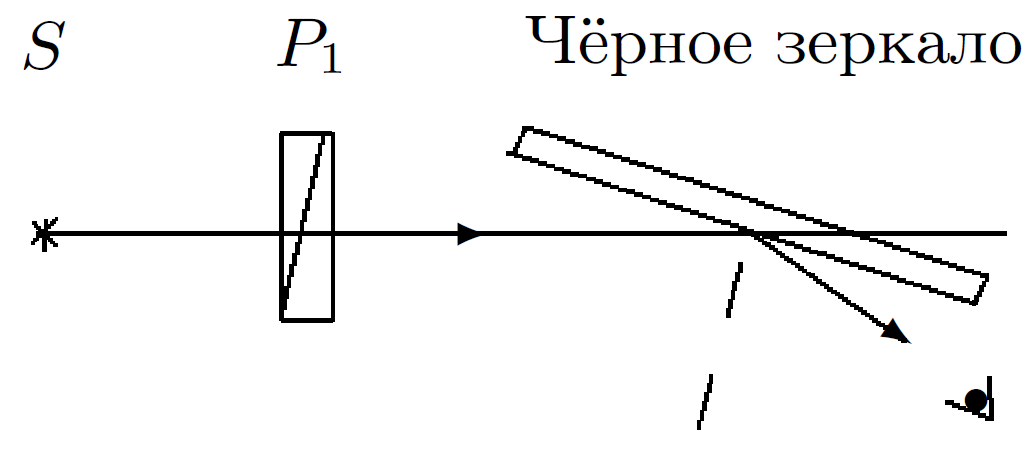
\includegraphics[width=6cm]{Screenshot_1.png}
	\caption{Определение разрешённых направлений поляроида.}
	\label{pic:1}
\end{wrapfigure}
Разместим па оптической скамье осветитель $ S $, поляроид $ P_1 $ и чёрное зеркало (пластинку чёрного стекла) так, чтобы плоскость падения была горизонтальна. Свет, отражённый от зеркала, рассматриваем сбоку, расположив глаз таким образом, чтобы вблизи оси вращения зеркала можно было увидеть изображение диафрагмы осветителя. Поворачивая поляроид вокруг направления луча, добьёмся наименьшей яркости отражённого пятна. Оставим поляроид в этом положении и вращением зеркала вокруг вертикальной оси снова добьёмся минимальной интенсивности отражённого луча.
Для первого поляроида разрешённое направление горизонтальное, на лимбе -10°
\\\\
Вместо чёрного зеркала поставим второй поляроид. Скрестим их, определим разрешённое направление второго поляроида --- вертикальная волна, на лимбе 75°

\subsection{Определение показателя преломления эбонита}
Поставим на скамью вместо чёрного зеркала эбонитовую пластину с круговой шкалой.
Повернем эбонитовое зеркало вокруг вертикальной оси так, чтобы его плоскость была перпендикулярна лучу, и попытаемся совместить отражённое от эбонита пятно с отверстием осветителя.
Установим направление разрешённых колебаний поляроида $ P_1 $ горизонтально и найдём угол поворота эбонита при котором интенсивность отражённого луча минимальна: его абсолютное значение равно $ 56^{\circ} \pm 5^{\circ} $
Повторим измерения, добавив светофильтр Ф, и сравним результаты --- они получились одинаковыми.
По углу Брюстера рассчитаем показатель преломления эбонита и сравним с табличным.
\begin{equation}\label{eq:1}
	n = \tg 56^{\circ} = 1,5 \pm 0,3
\end{equation}
Табличное значение показателя преломления эбонита $ n = 1.6 $
\newpage
\subsection{Исследование стопы}
\begin{wrapfigure}{r}{5.5cm}
	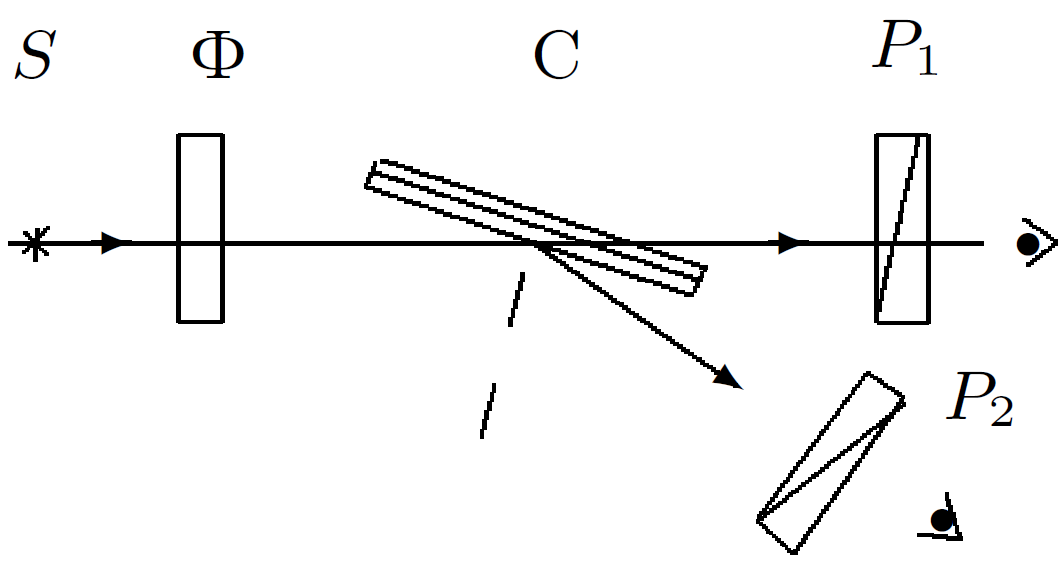
\includegraphics[width=5.5cm]{Screenshot_2.png}
	\caption{Исследование стопы.}
	\label{pic:2}
\end{wrapfigure}
Поставим стопу стеклянных пластинок вместо эбонитового зеркала и подберем для неё такое положение, при котором свет падает на стопу под углом Брюстера. Осветим стопу неполяризованным светом и, рассматривая через поляроиды свет, отражённый от стопы, определим ориентацию вектора $ \mathbf{E} $ в отражённом луче; затем определим характер поляризации света в преломлённом луче. Получаем, что преломленные лучи \underline{горизонтальные}, отраженные \underline{вертикальные}.

\subsection{Определение главных плоскостей двоякопреломляющих пластин}
\begin{wrapfigure}{r}{5.5cm}
	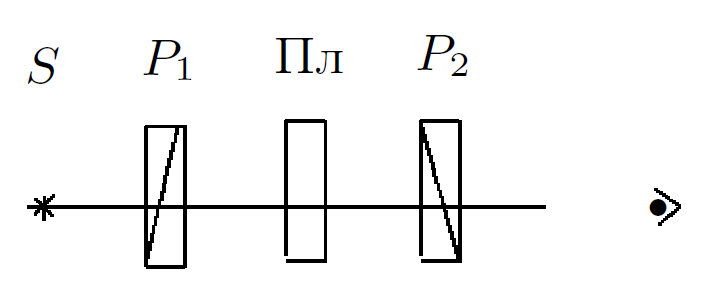
\includegraphics[width=5.5cm]{Screenshot_3.png}
	\caption{Определение главных направлений в пластинках.}
	\label{pic:3}
\end{wrapfigure}
Поставим кристаллическую пластинку между скрещенными поляроидами $ P_1 $ и $ P_2 $. Вращая пластинку вокруг направления луча и наблюдая за интенсивностью света, проходящего сквозь второй поляроид, определим, при каком условии главные направления пластинки совпадают с разрешёнными направлениями поляроидов. Повторим опыт для второй пластинки. Минимумы и максимумы интенсивности чередуются через 45°, главные плоскости пластин совпадают с разрешенными направлениями поляроидов при максимальной интенсивности. Максимумы: для первой \underline{$ \alpha_0 = 28 $°}, для второй \underline{$ \alpha_0 = 6 $°}.

\subsection{Выделение пластин $ \lambda / 2 $ и $ \lambda / 4 $}
Для выделения пластин $ \lambda / 2 $, $ \lambda / 4 $. Добавим к схеме, изображённой на рис. 2, зелёный фильтр и установим разрешённое направление первого поляроида горизонтально, а главные направления исследуемой пластинки -- под углом 45° к горизонтали. Для первой получаем, что после поворота свет становится фиолетовым и тускнеет, следовательно линейная поляризация и пластинка $ \lambda / 2 $. Для второй: свет становится зелёным и не тускнеет, следовательно круговая поляризация и пластинка $ \lambda / 4 $.

\subsection{Быстрая и медленная оси $ \lambda / 4 $}
\begin{wrapfigure}{r}{5.5cm}
	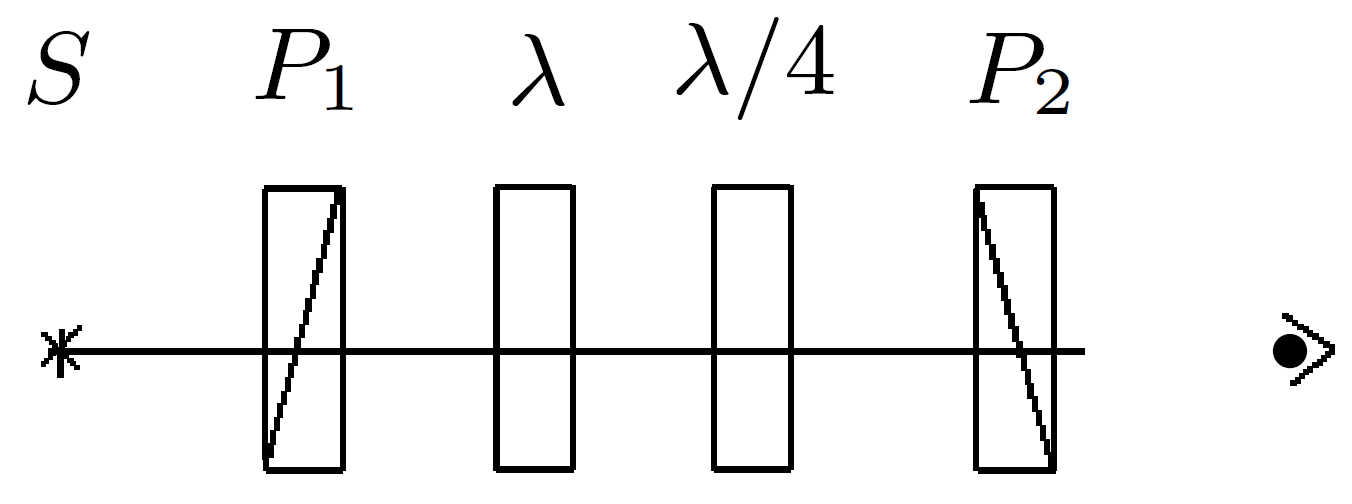
\includegraphics[width=5.5cm]{Screenshot_4.png}
	\caption{Определение направлений большей и меньшей скорости}
	\label{pic:4}
\end{wrapfigure}
Определим «быструю» и «медленную» оси в пластинке $ \lambda / 4 $.
\\
Поставим между скрещенными поляроидами пластинку чувствительного оттенка, имеющую вид стрелки, и убедимся, что эта пластинка не меняет поляризацию зелёного света. Уберем зелёный фильтр и убедимся, что стрелка имеет пурпурный цвет. Это объясняется тем, что зелёная компонента линейно поляризованного света при прохождении пластинки не меняет поляризации и задерживается вторым поляроидом.
\\
Добавим к схеме пластинку $ \lambda / 4 $ (рис. 4), главные направления которой совпадают с главными направлениями пластины $ \lambda $ и ориентированы под углом 45° к разрешённым направлениям скрещенных поляроидов. При повороте рейтера со стрелкой на 180° вокруг вертикальной оси цвет стрелки меняется от зелёно-голубого до оранжево-жёлтого. В первом случае у нас «быстрая» ось (они совпадают), во втором -- медленная.

\subsection{Интерференция поляризованных лучей}
Исследуем интерференцию поляризованных лучей. Для этого расположим между скрещенными поляроидами мозаичную слюдяную пластинку. Она собрана из 4-х узких полосок слюды, лежащих по сторонам квадрата (две полоски «толщиной» $ \lambda / 4 $ и но одной — $ \lambda / 2 $ и $ 3 \lambda / 4 $). В центральном квадратике слюды нет. Главные направления всех пластинок ориентированы параллельно сторонам квадрата.
\\\\
Вращая пластинку, пронаблюдаем за изменениями в отдельном квадратике. У нас изменяется интенсивность.
\\\\
Не трогая пластинки, повращаем второй поляроид. Отличие в том, что теперь изменяется цвет.

\subsection{Определение направления вращения светового вектора в эллиптически поляризованной волне}

\begin{figure}[H]
	\center{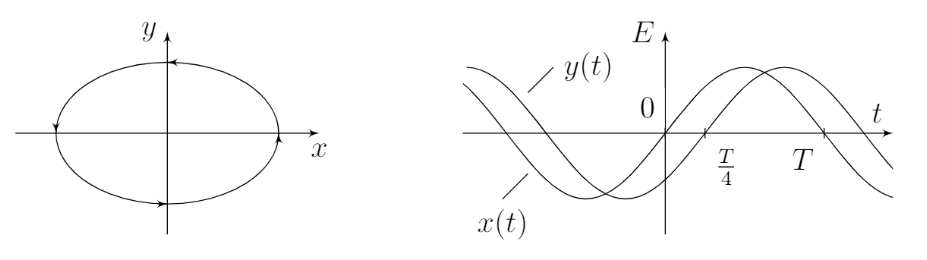
\includegraphics[scale=0.7]{Screenshot_5.png}}
	\caption{\centering Эллипс поляризации и графики синусоид.}
	\label{pic:5}
\end{figure}
Снова поставим зеленый фильтр, а за ним между скрещенными поляроидами -- пластинку произвольной толщины $( \lambda / 4 )$.
\\\\
Получим эллиптически-поляризованный свет. Для этого установим разрешённое направление первого поляроида под углом 10°--20° к горизонтали так, чтобы вектор \textbf{E} падающего на пластинку света был расположен в первом квадранте. Установим разрешённое направление второго поляроида вертикально и, вращая пластинку, найдем минимальную интенсивность света, прошедшего второй поляроид. Вращая второй поляроид, убедитесь, что свет поляризован эллиптически, а нс линейно. Таким образом, получим эллипс поляризации с вертикально ориентированной малой осью.
\\\\
Для определения направления вращения светового вектора в эллипсе установим между поляроидами дополнительную пластинку $ \lambda / 4 $ с известными направлениями «быстрой» и «медленной» осей, ориентированными по осям эллипса поляризации анализируемого света. В этом случае вектор \textbf{E} на выходе будет таким, как если бы свет прошел две пластинки $ \lambda / 4 $: свет на выходе из второй пластинки будет линейно поляризован. Если пластинки поодиночке дают эллипсы, вращающиеся в разные стороны, то поставленные друг за другом, они скомпенсируют разность фаз, и вектор \textbf{E} на выходе останется в первом и третьем квадрантах. Если же световой вектор перешёл в смежные квадранты, значит, эллипсы вращаются в одну сторону.
\\\\
После второго поляроида интенсивность света максимальна в первом квадранте. Значит, две пластины компенсируют друг друга, световой вектор остался в том же квадранте, эллипсы вращаются в разные сторону.

\section{Вывод}
Таким образом, в ходе работы были получены следующие результаты:
\begin{itemize}
\item Определены разрешённые направления поряроидов --- для первого поляроида разрешённое направление горизонтальное, на лимбе $-10^{\circ}$, для второго поляроида --- вертикальная волна, на лимбе $75^{\circ}$;
\item Был определен показатель преломления эбонита по углу Брюстера:
\begin{equation*}
    n = \tg{56^{\circ}} = 1,5 \pm 0,6
\end{equation*}
Полученный результат в пределах погрешности совпадает с табличным $n = 1,6$;
\item Получили, что в стопе стеклянных пластинок преломленные лучи горизонтальные, а отраженные --- вертикальные;
\item Для двоякопреломляющих пластин определены главные направления --- минимумы и
максимумы интенсивности чередуются через $45^{\circ}$, главные плоскости пластин совпадают с разрешенными направлениями поляроидов при максимальной интенсивности. Максимумы: для первой $\alpha_0 = 28^{\circ}$, для второй $\alpha_0 = 6^{\circ}$;
\item Выяснили, что из двух имеющихся пластинок первая из них --- пластинка $\lambda/2$, а вторая --- $\lambda/4$;
\item «Быстрая» ось пластинки $\lambda/4$ совпадает с «быстрой» осью пластинки $\lambda$ и ориентирована под углом $45^{\circ}$ к разрешенным направлениям скрещенных поляроидов. При повороте рейтера со стрелкой на $180^{\circ}$ вокруг вертикальной оси получаем медленную ось.
\item При изучении интерференции поляризованных лучей было получено, что при вращении пластинки в отдельном квадратике изменяется интенсивность, а при вращении второго поляроида --- изменяется цвет;
\item Было определено направление вращения светового вектора в эллиптически поляризованной волне после пластинки $\lambda/4$: оно компенсирует разность фаз со второй пластинкой, «быстрая» и «медленная» оси которой известны. Таким образом, эллипс первой пластинки вращается в противоположную сторону.
\end{itemize}

\end{document}